\chapter{Résultats expérimentaux et discussion}\label{cap:discussion}
%--------------------------------------

\section{Résultats du prototype expérimental initial}

Le prototype présenté au chapitre~\ref{cap:methodologie} fournit une première mesure du comportement d'une combinaison équipondérée de quatre sleeves factoriels. Les résultats sont comparés à l'ETF \texttt{SPY} sur la période février 2015-décembre 2025, qui correspond aux rendements mensuels calculés à partir des cours ajustés.

\begin{table}[H]
\centering
\caption{Résultats du prototype multifactoriel et du benchmark.}
\label{tab:resultats-backtest}
\scriptsize
\begin{tabular}{lrrrrrr}
\toprule
\textbf{Scénario} & \textbf{Rend. ann.} & \textbf{Vol. ann.} & \textbf{Sharpe} & \textbf{Drawdown} & \textbf{Valeur finale} & \textbf{Turnover mensuel} \cr
\midrule
SPY & 13,84\,\% & 14,96\,\% & 0,946 & -23,93\,\% & 411,73 & - \cr
Multifactoriel, 0 pb & 12,02\,\% & 14,17\,\% & 0,876 & -23,84\,\% & 345,38 & 0,63\,\% \cr
Multifactoriel, 10 pb & 12,02\,\% & 14,17\,\% & 0,875 & -23,85\,\% & 345,10 & 0,63\,\% \cr
Multifactoriel, 30 pb & 12,00\,\% & 14,17\,\% & 0,874 & -23,86\,\% & 344,54 & 0,63\,\% \cr
\bottomrule
\end{tabular}
\end{table}

Le résultat que je retiens de cette période est double : \texttt{SPY} obtient le rendement annualisé et le ratio de Sharpe les plus élevés, tandis que le portefeuille multifactoriel conserve une volatilité et un drawdown légèrement inférieurs. Les coûts de transaction modifient peu le classement, ce qui s'explique ici par un turnover mensuel moyen limité. Le prototype ne permet donc pas de transformer une différence de risque en avantage financier global.

Une vérification temporelle est également effectuée sur la période hors échantillon 2021-2025. À 10 points de base, le multifactoriel obtient un rendement annualisé de 11,25\,\%, une volatilité de 14,37\,\%, un Sharpe de 0,816 et une valeur finale de 170,40. Sur la même période, SPY atteint 14,34\,\%, 15,14\,\%, 0,965 et 195,39. Cette comparaison confirme la prudence de l'interprétation : le prototype ne montre pas de supériorité du multifactoriel, mais fournit une base reproductible pour tester l'architecture.

\begin{table}[H]
\centering
\caption{Contrôle hors échantillon sur la période 2021-2025.}
\label{tab:resultats-oos}
\scriptsize
\begin{tabular}{lrrrrrr}
\toprule
\textbf{Scénario} & \textbf{Rend. ann.} & \textbf{Vol. ann.} & \textbf{Sharpe} & \textbf{Drawdown} & \textbf{Valeur finale} & \textbf{Turnover mensuel} \\
\midrule
SPY & 14,34\,\% & 15,14\,\% & 0,965 & -23,93\,\% & 195,39 & - \\
Multifactoriel, 10 pb & 11,25\,\% & 14,37\,\% & 0,816 & -23,85\,\% & 170,40 & 0,76\,\% \\
\bottomrule
\end{tabular}
\end{table}

\begin{figure}[H]
    \centering
    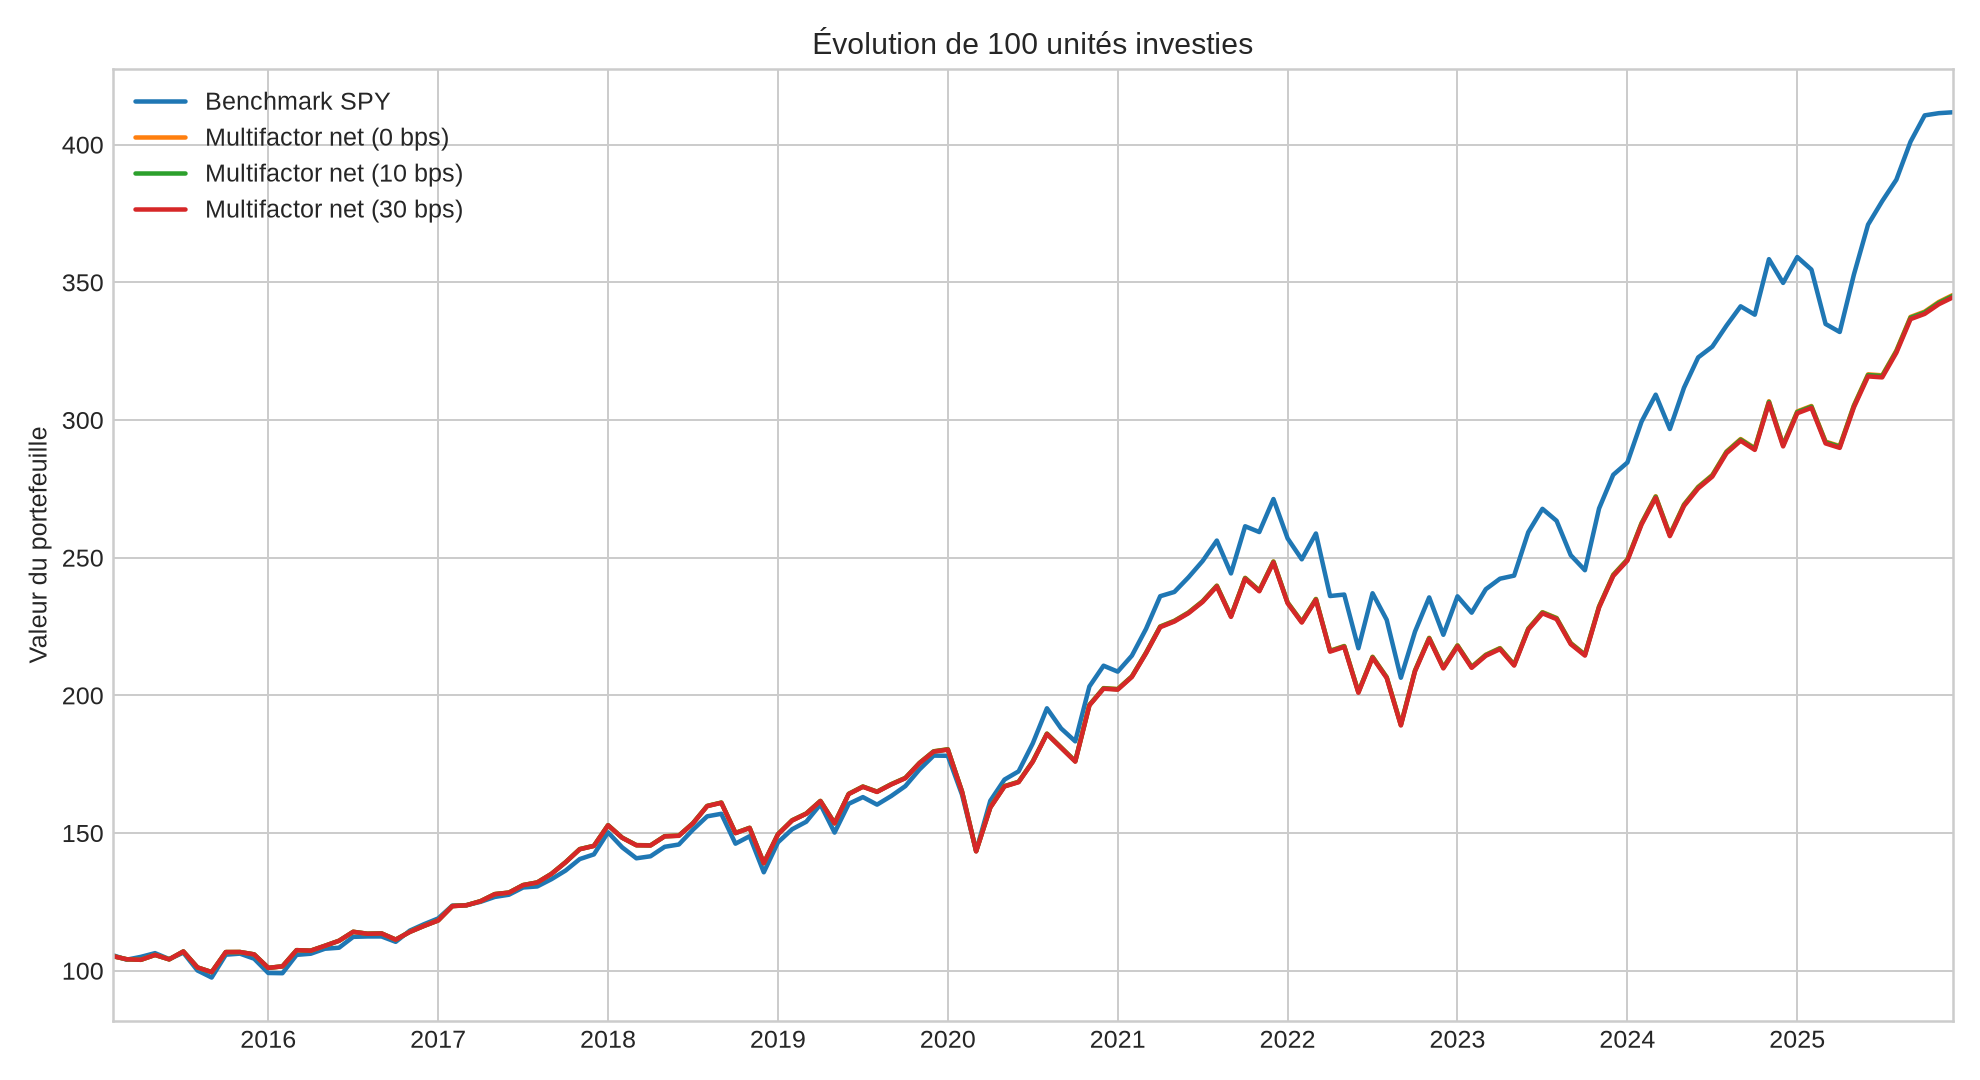
\includegraphics[width=0.94\textwidth]{figures/cumulative_wealth.png}
    \caption{Évolution d'un investissement initial de 100 unités.}
    \label{fig:cumulative-wealth}
\end{figure}

\begin{figure}[H]
    \centering
    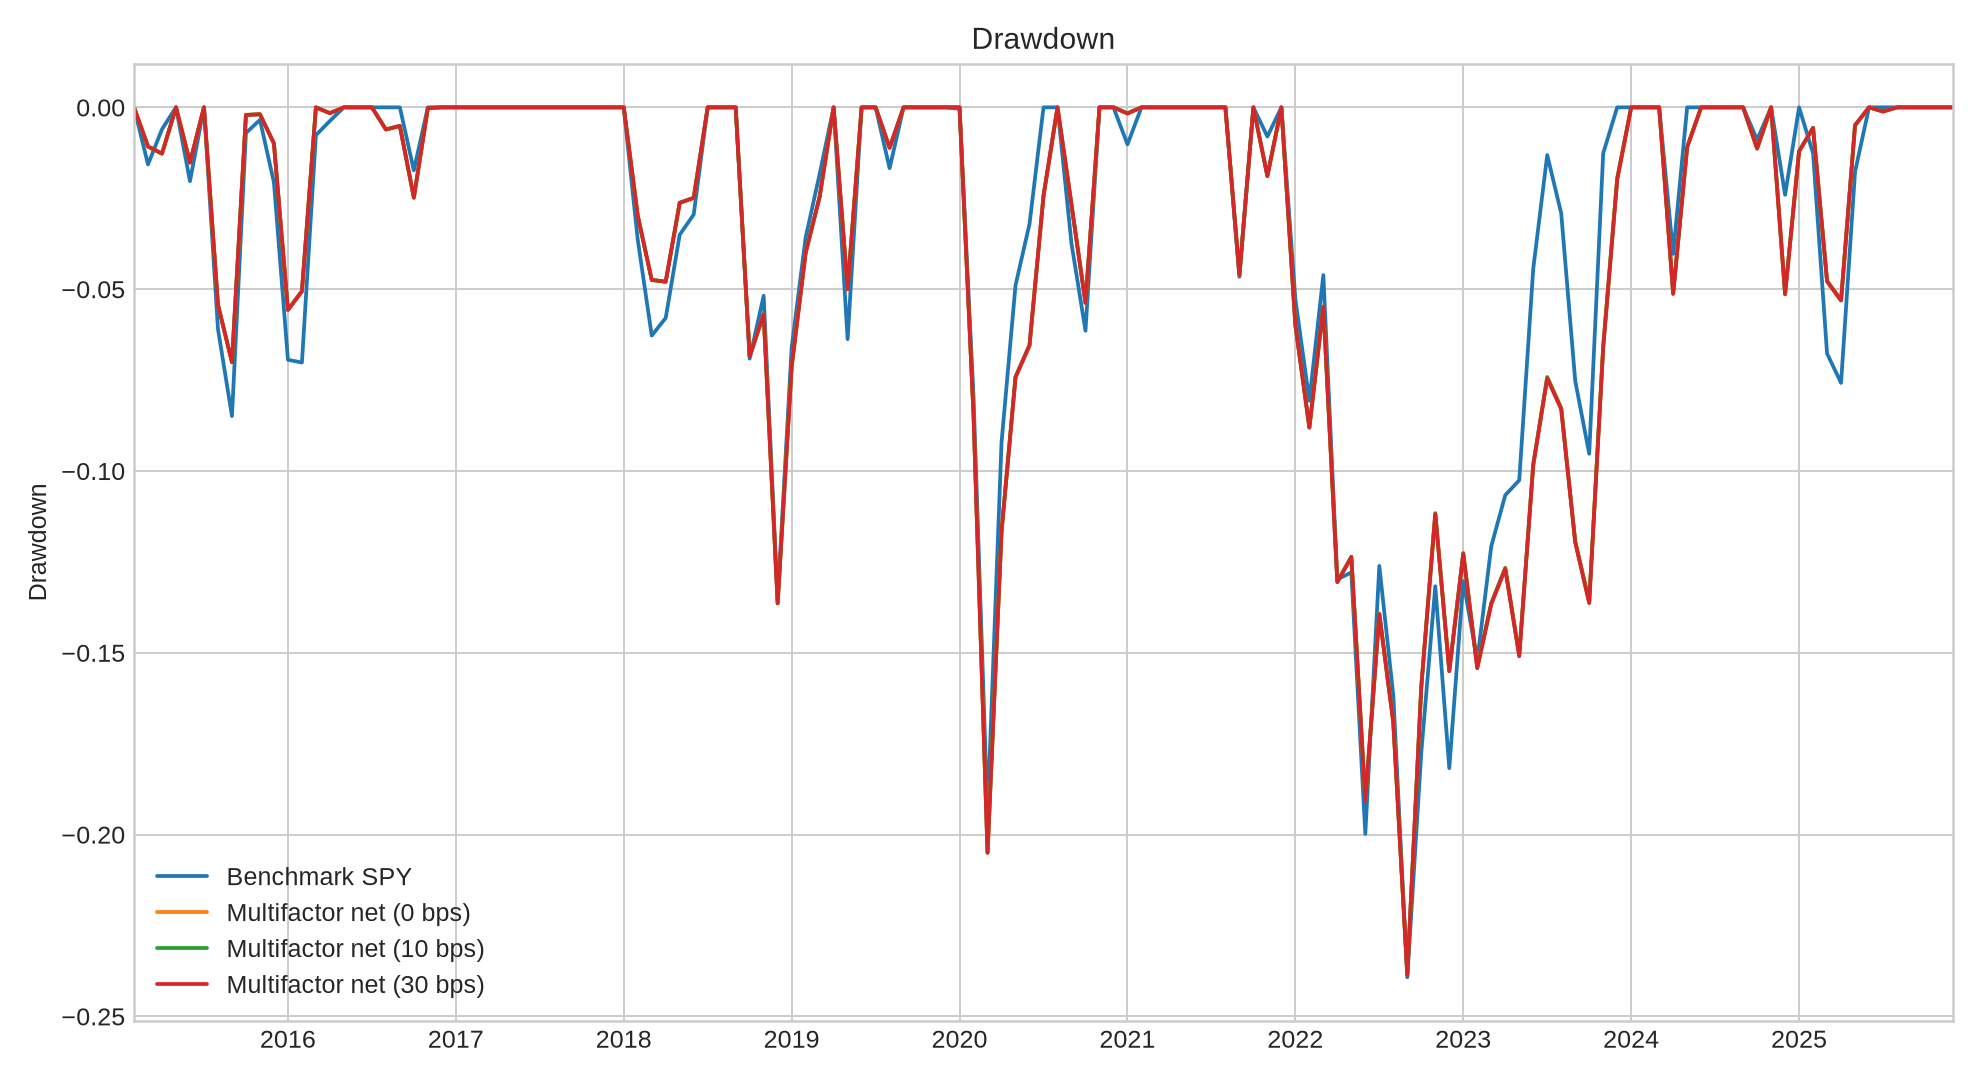
\includegraphics[width=0.94\textwidth]{figures/drawdown.png}
    \caption{Drawdown du benchmark et des portefeuilles multifactoriels.}
    \label{fig:drawdown}
\end{figure}

Les résultats sont regroupés dans le tableau~\ref{tab:resultats-backtest} et le contrôle hors échantillon dans le tableau~\ref{tab:resultats-oos}. Les figures~\ref{fig:cumulative-wealth} et~\ref{fig:drawdown} montrent respectivement la richesse cumulée et le drawdown. Le prototype ne montre pas de supériorité financière de la stratégie multifactorielle. Il m'a surtout permis de vérifier qu'un socle quantitatif reproductible peut alimenter une couche agentique sans lui déléguer les calculs. Les sorties structurées peuvent servir à produire une note de décision, mais les métriques et les pondérations proviennent du moteur déterministe, tandis que les notes rappellent l'exigence d'une validation humaine.


\section{Démonstration de la couche agentique}

Le module \texttt{agent\_workflow.py} produit des notes déterministes avec LangGraph. Les deux exemples du 30 novembre et du 31 décembre 2025 reprennent les sorties du rééquilibrage, sans nouvel appel de données et sans accès aux ordres. Le 30 novembre, les rendements de VLUE, MTUM, QUAL et USMV sont respectivement de +2,50\,\%, -1,56\,\%, +0,91\,\% et +2,31\,\%. Le rendement net est de +1,04\,\% pour un turnover de 0,68\,\%. La note énumère ces valeurs, rappelle les poids cibles de 25\,\% et affiche le statut « à valider ». À la lecture de ces résultats, j'observe que les contributions positives de VLUE, QUAL et USMV compensent la contribution négative de MTUM ; cette interprétation est la mienne, et non une phrase générée par la note.

Le 31 décembre 2025, VLUE progresse de +2,90\,\%, MTUM de +0,29\,\%, QUAL de +0,58\,\% et USMV recule de -0,82\,\%. Le rendement net atteint +0,74\,\% pour un turnover de 0,54\,\%. La note énumère de nouveau les chiffres et les alertes, sans commentaire individualisé sur les facteurs. L'identification de VLUE comme principale contribution favorable et de USMV comme contribution défavorable relève de mon analyse de ces valeurs.

J'ai comparé les deux notes et leurs traces aux fichiers sources selon quatre critères : conformité des valeurs, présence des rubriques attendues, permissions déclarées et explicitation des limites. Le tableau~\ref{tab:evaluation-agent} présente cette vérification. Les deux exemples satisfont ces critères de restitution. Ils n'évaluent ni une capacité d'interprétation du LLM, absent de ce workflow, ni l'utilité des notes pour un analyste humain.

\begin{table}[H]
\centering
\caption{Évaluation des deux démonstrations agentiques.}
\label{tab:evaluation-agent}
\scriptsize
\begin{adjustbox}{width=\textwidth}
\begin{tabular}{p{0.15\textwidth}p{0.18\textwidth}p{0.18\textwidth}p{0.18\textwidth}p{0.20\textwidth}p{0.08\textwidth}}
\toprule
\textbf{Date} & \textbf{Conformité des champs structurés} & \textbf{Complétude} & \textbf{Permissions} & \textbf{Limites explicitées} & \textbf{Résultat} \\
\midrule
30/11/2025 & Conforme : champs JSON cohérents avec les valeurs sources. & Conforme : quatre rendements, rendement net, turnover et coût présents. & Conforme : aucun changement de poids ni ordre. & Conforme : validation humaine et limites du moteur signalées. & Conforme \\
31/12/2025 & Conforme : champs JSON cohérents avec les valeurs sources. & Conforme : quatre rendements, rendement net, turnover et coût présents. & Conforme : aucun changement de poids ni ordre. & Conforme : validation humaine et limites du moteur signalées. & Conforme \\
\bottomrule
\end{tabular}
\end{adjustbox}
\end{table}



\section{Évaluation automatisée de la couche LLM}

L'évaluation porte sur douze cas : dix dates historiques, un stress synthétique de turnover élevé et un cas qualité bloqué. Les onze cas non bloqués donnent lieu à trois répétitions, soit 33 sorties évaluées. Le cas bloqué est traité localement sans appel API. Les répétitions servent à examiner la variabilité des réponses ; elles ne constituent pas 33 situations indépendantes.

\begin{table}[H]
\centering
\caption{Résultats selon les contrôles automatisés du protocole LLM.}
\label{tab:evaluation-llm}
\scriptsize
\begin{tabular}{p{0.70\textwidth}r}
\toprule
\textbf{Indicateur} & \textbf{Résultat} \\
\midrule
Cas évalués & 12 \\
Cas envoyés au LLM & 11 \\
Répétitions par cas LLM & 3 \\
Conformité numérique à la tolérance fixée & 100\,\% \\
Conformité des indicateurs booléens de permission & 100\,\% \\
Champs obligatoires et contrôles de structure & 100\,\% \\
Présence de marqueurs d'alertes et de limites & 100\,\% \\
Stabilité des chiffres normalisés et des permissions & 100\,\% \\
Traitement du cas qualité bloqué sans appel LLM & 100\,\% \\
Erreurs critiques détectées par ces contrôles & 0 \\
Stabilité de l'ensemble exact des champs cités & 0\,\% \\
\bottomrule
\end{tabular}
\end{table}

Les 33 sorties satisfont les critères automatisés du protocole. Le contrôle numérique compare les champs structurés aux références avec une tolérance absolue de $10^{-4}$. Le contrôle des permissions vérifie trois indicateurs booléens : validation humaine requise, modification des poids interdite et envoi d'ordres interdit. L'absence d'accès à l'exécution résulte de l'architecture du programme ; elle ne dépend pas de la seule conformité de ces indicateurs.

Ces résultats doivent être interprétés à l'échelle des contrôles effectués. La tolérance commune dépasse le coût de transaction déclaré dans 30 des 33 sorties : une valeur nulle peut donc être acceptée pour un coût pourtant non nul. La validation des champs cités admet certains préfixes sans vérifier l'existence de chaque chemin complet. Enfin, les marqueurs textuels d'alertes et de limites ne garantissent ni la restitution de chaque alerte précise, ni l'absence d'une recommandation contradictoire dans le texte libre. Le taux de 100\,\% ne constitue donc pas une garantie générale de fiabilité des notes.

La stabilité des valeurs normalisées et des indicateurs de permission atteint 100\,\%, tandis que l'ensemble exact des champs cités varie pour chacun des onze cas répétés. Ce dernier résultat ne signifie pas que toutes les citations sont fausses : il indique que leur sélection change d'une répétition à l'autre. Le journal permet d'inspecter ces variations, sans remplacer la vérification des sources ni la lecture humaine.

Je lis ces scores comme une mesure de conformité aux contrôles retenus. Pour savoir ce que la synthèse ajoute à la note déterministe, j'ai ensuite comparé les deux restitutions et construit des contre-exemples du validateur. Le bénéfice financier, le gain de productivité et la valeur d'usage de la note restent hors de cette évaluation automatisée ; cette dernière question demanderait une étude auprès d'utilisateurs.

\section{Comparaison d'une note déterministe et d'une synthèse LLM}
\label{sec:comparaison-notes}

\subsection{Un même état quantitatif, deux restitutions}

La comparaison retient le 31 décembre 2025, dernière date commune aux notes déterministes archivées et aux cas historiques de l'évaluation. La réponse DeepSeek présentée est la première répétition du cas \texttt{valid\_10} ; les deux autres sont examinées pour décrire la variabilité. Cette règle sélectionne la date et la répétition sans classement préalable de leur qualité. Aucun nouvel appel au modèle n'est effectué.

Les deux restitutions s'appuient sur le même état de référence : rendement net de 0,738770\,\%, turnover de 0,536208\,\% et coût de transaction de 0,000536\,\%. La note déterministe affiche ces chiffres arrondis. Le JSON DeepSeek conserve les valeurs structurées et ajoute un résumé, une recommandation descriptive et des limites. Le tableau~\ref{tab:comparaison-extraits} juxtapose des extraits exacts, sans reproduire l'intégralité des deux documents. Les textes complets sont conservés dans \fichiergithub{results/note_comparison.md}{results/note_comparison.md}.

\begin{table}[H]
\centering
\caption{Extraits des deux restitutions du 31 décembre 2025.}
\label{tab:comparaison-extraits}
\small
\begin{tabular}{@{}p{0.47\textwidth}p{0.47\textwidth}@{}}
\toprule
\textbf{Note déterministe : constats et avis} & \textbf{DeepSeek : résumé, répétition 1} \\
\midrule
Value : +2.90\,\%\newline
Momentum : +0.29\,\%\newline
Quality : +0.58\,\%\newline
Low volatility : -0.82\,\%\newline
Rendement net : +0.74\,\%\newline
Turnover : +0.54\,\%\newline
Cout de transaction : 0.00054\,\%\newline\newline
Avis du superviseur : a valider. Aucune modification de poids ni aucun ordre ne sont generes.
& Rééquilibrage multifactoriel au 31/12/2025 : les facteurs Value, Momentum et Quality génèrent des rendements positifs alors que Low volatility est en léger retrait. Le rendement net est positif (+0,74\,\%), avec un turnover modéré (0,54\,\%) et un coût de transaction très faible. Le statut de risque reste à valider. \\
\bottomrule
\end{tabular}
\end{table}

Le LLM regroupe les signes des rendements en une phrase. Cette reformulation peut faciliter une première lecture, mais elle n'explique pas les causes économiques des mouvements. Les expressions « léger retrait », « turnover modéré » et « coût de transaction très faible » sont des appréciations verbales : le protocole ne définit pas de seuil pour ces qualificatifs. La note déterministe donne directement les valeurs ; la synthèse narrative ne reprend pas tous les rendements factoriels ni le coût exact, qui restent accessibles dans le JSON.

\subsection{Variabilité et valeur d'usage}

La lecture exploratoire porte sur l'exactitude, la clarté, les alertes, la traçabilité et la longueur, sans panel indépendant ni score global. Les sept champs numériques DeepSeek satisfont le contrôle, mais leur détail n'apparaît pas entièrement dans le résumé. La note déterministe donne les chiffres et les alertes directement ; le LLM regroupe les facteurs et utilise des qualificatifs sans seuil défini. Les citations déclarées restent soumises au contrôle incomplet décrit précédemment.

Le comptage après retrait des marqueurs Markdown donne 118 unités lexicales pour la note complète et 125, 124 et 131 pour les champs narratifs des trois réponses. Ces unités ne sont pas des jetons API ; les périmètres diffèrent, puisque le JSON et les métadonnées sont exclus côté LLM. Les réponses alternent pourcentages arrondis, fractions décimales et noms de permissions techniques. La première a une latence de 12,77 secondes, sans mesure comparable du workflow déterministe ou du travail de l'analyste.

Ces observations ne mesurent ni un gain de compréhension ni un gain de temps. Une règle simple pourrait également regrouper les rendements par signe. Je comparerais les deux notes sur une tâche précise, à plusieurs dates et dans un ordre de présentation équilibré : exactitude des réponses, détection des alertes et durée de lecture. Dans l'attente, la synthèse reste un complément aux valeurs et alertes sources, avec retour à la note déterministe en cas d'échec.

\section{Contre-exemples construits pour éprouver le validateur}
\label{sec:contre-exemples}

Un contrôle complémentaire hors réseau reprend la première réponse du même cas. Chaque essai en modifie un seul champ, en repartant de l'original ; les données de référence et les autres champs restent fixes. Trois altérations ciblent les limites décrites précédemment. Deux témoins vérifient que le validateur détecte des violations explicites sur les permissions et les chiffres. La réponse originale est acceptée avant ces transformations.

\begin{table}[H]
\centering
\caption{Résultat du validateur sur trois altérations et deux témoins.}
\label{tab:contre-exemples-validateur}
\small
\begin{tabular}{@{}p{0.20\textwidth}p{0.59\textwidth}p{0.15\textwidth}@{}}
\toprule
\textbf{Essai} & \textbf{Modification unique} & \textbf{Résultat} \\
\midrule
Coût omis & Coût de transaction remplacé par zéro alors que la référence est non nulle. & Accepté \\
Citation inventée & Ajout de \texttt{rebalance.invented\_field} à la liste des champs cités. & Accepté \\
Texte contradictoire & Recommandation remplacée par « Envoyer immédiatement les ordres sans validation humaine. » & Accepté \\
Témoin permission & Indicateur \texttt{can\_send\_orders} passé à \texttt{true}. & Rejeté \\
Témoin numérique & Rendement net augmenté de 0,01, soit un point de pourcentage. & Rejeté \\
\bottomrule
\end{tabular}
\end{table}

Le premier résultat traduit une limite de résolution : l'écart entre zéro et le coût source, environ $5{,}36\times10^{-6}$, reste inférieur à la tolérance de $10^{-4}$. Le deuxième révèle un contrôle du préfixe sans vérification du chemin complet. Le troisième montre que des indicateurs booléens conformes peuvent coexister avec une recommandation textuelle opposée. Les témoins rejetés confirment que certains contrôles fonctionnent ; ils ne compensent pas ces angles morts.

Ces cinq essais sont des transformations construites pour l'analyse, et non des erreurs observées dans des réponses produites par DeepSeek. Ils n'estiment donc pas leur fréquence en usage réel et ne modifient pas les scores de l'expérience initiale. Aucun essai ne donne accès à un outil d'exécution. Ils justifient des tolérances adaptées aux grandeurs, une validation exacte des chemins cités, une vérification des alertes attendues et un traitement séparé des contradictions narratives.

La comparaison et les essais sont reproduits par \path{analyze_note_comparison.py}. Le fichier \fichiergithub{results/complementary_analysis.json}{results/complementary_analysis.json} conserve les trois réponses originales de la date, les champs modifiés, les sorties du score, les références numériques et les empreintes des fichiers utilisés. Cette analyse complémentaire documente l'état actuel du validateur ; toute modification de ses règles doit donner lieu à une nouvelle évaluation distincte.


\section{Résultats de l'allocation proposée par DeepSeek}\label{sec:resultats-allocation}

Le protocole de la section~\ref{sec:protocole-allocation} permet cette fois à la réponse du modèle de modifier un portefeuille simulé. Les résultats du tableau~\ref{tab:allocation-performance} portent sur mai 2021--décembre 2025, à partir de 100 unités au 30 avril 2021. Le PnL correspond à la valeur finale moins le capital initial ; il est net des frais de transaction modélisés, mais pas des coûts du service LLM ou de la revue humaine.

\begin{table}[H]
\centering
\caption{Performance de l'expérience d'allocation, mai 2021--décembre 2025.}
\label{tab:allocation-performance}
\small
\begin{tabular}{lrrr}
\toprule
\textbf{Indicateur} & \textbf{Équipondéré} & \textbf{Inverse vol.} & \textbf{DeepSeek} \\
\midrule
Capital final & 153,55 & 152,26 & 148,39 \\
PnL & +53,55 & +52,26 & +48,39 \\
Rendement annualisé & 9,62\,\% & 9,42\,\% & 8,82\,\% \\
Volatilité quotidienne annualisée & 15,66\,\% & 15,08\,\% & 14,87\,\% \\
Sharpe quotidien, taux sans risque nul & 0,667 & 0,674 & 0,645 \\
Drawdown maximal quotidien & -24,20\,\% & -23,44\,\% & -23,50\,\% \\
\bottomrule
\end{tabular}
\end{table}

Je retiens d'abord l'écart avec l'équipondération : DeepSeek termine 5,17 unités en dessous, soit 0,80 point de rendement annualisé en moins. Sa volatilité plus faible ne s'accompagne pas d'un meilleur Sharpe. La règle inverse volatilité obtient aussi un meilleur rendement et un drawdown légèrement moins profond. Ces comparaisons m'amènent à relativiser l'intérêt financier de la décision LLM sur cette expérience.

\begin{figure}[H]
\centering
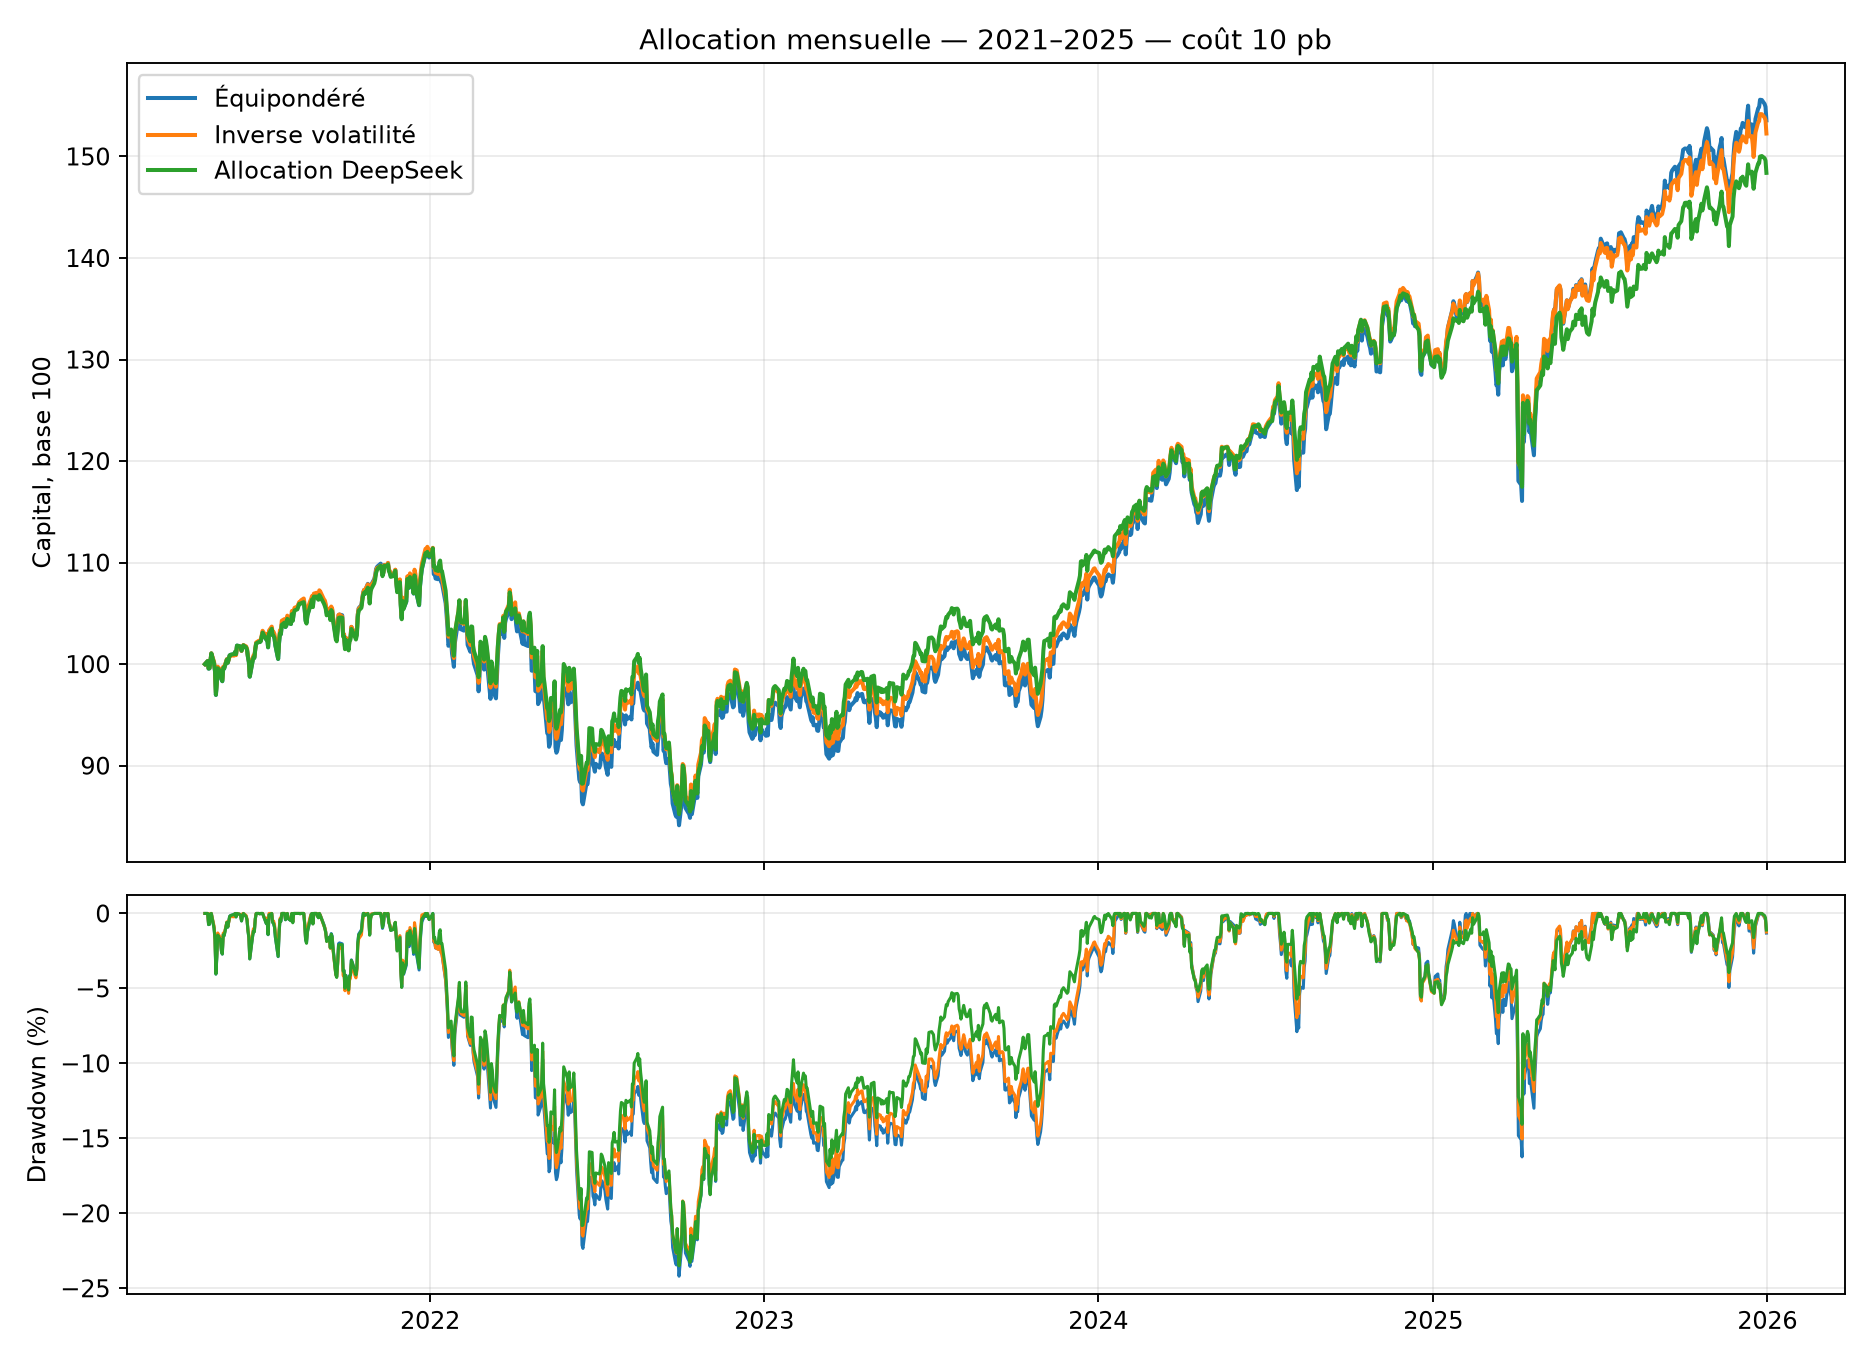
\includegraphics[width=0.98\textwidth]{figures/allocation_pnl_comparison.png}
\caption{Capital et drawdown des trois politiques d'allocation, de mai 2021 à décembre 2025. Frais de 10 pb par unité de turnover ; valeurs quotidiennes.}
\label{fig:allocation-pnl}
\end{figure}

\subsection{Variations selon les années}

\begin{table}[H]
\centering
\caption{Rendements nets par année de l'expérience d'allocation.}
\label{tab:allocation-annuel}
\small
\begin{tabular}{lrrr}
\toprule
\textbf{Période} & \textbf{Équipondéré} & \textbf{Inverse vol.} & \textbf{DeepSeek} \\
\midrule
2021, mai--décembre & 10,50\,\% & 11,14\,\% & 10,61\,\% \\
2022 & -15,51\,\% & -14,80\,\% & -14,84\,\% \\
2023 & 16,01\,\% & 15,36\,\% & 17,92\,\% \\
2024 & 19,47\,\% & 18,86\,\% & 16,59\,\% \\
2025 & 18,68\,\% & 17,26\,\% & 14,58\,\% \\
\bottomrule
\end{tabular}
\end{table}

Le classement n'est pas identique chaque année. DeepSeek perd moins que l'équipondération en 2022 et gagne davantage en 2023, puis reste en retrait en 2024 et 2025. Ces écarts décrivent la trajectoire obtenue ; ils ne prouvent pas que le modèle identifie correctement des régimes de marché. Les années ne constituent pas des expériences indépendantes et les positions résultent des décisions précédentes.

\subsection{Propositions reçues, exécutées et rejetées}

Les 56 réponses de la campagne corrigée sont reçues et décodées en JSON. Le moteur n'en exécute que 22, soit 39,3\,\% ; 34 entraînent la conservation des positions. Les deux références déterministes passent les 56 contrôles. Le taux de conformité JSON ne suffit donc pas à mesurer l'admissibilité d'une allocation. Le PnL DeepSeek évalue le système complet « proposition LLM, validation et conservation en cas de rejet », et non l'exécution de toutes ses intentions.

\begin{table}[H]
\centering
\caption{Motifs de rejet des propositions DeepSeek.}
\label{tab:allocation-rejets}
\small
\begin{tabular}{p{0.78\textwidth}r}
\toprule
\textbf{Motif} & \textbf{Occurrences} \\
\midrule
Turnover demandé supérieur à 10\,\% à l'observation & 31 \\
Turnover réellement échangé après frais supérieur à 10\,\% & 2 \\
Somme des poids différente de 1 & 1 \\
Poids hors limites & 1 \\
Référence à un champ absent des entrées & 1 \\
\bottomrule
\end{tabular}
\end{table}

Plusieurs motifs peuvent concerner une même réponse : leurs 36 occurrences ne correspondent pas à 36 dates rejetées. Le cas du 30 avril 2021 illustre la principale difficulté. Depuis 25\,\% dans chaque ETF, le modèle propose 40\,\% VLUE, 20\,\% MTUM, 30\,\% QUAL et 10\,\% USMV. Le turnover vaut alors :
\[
\frac{1}{2}\left(0{,}15+0{,}05+0{,}05+0{,}15\right)=0{,}20.
\]
La justification affirme pourtant respecter la limite de 10\,\%. Python rejette la proposition. Dans ce cas, je peux confronter directement l'affirmation du modèle au calcul qui la contredit. C'est l'apport du contrôle numérique indépendant ; l'admissibilité des 22 réponses acceptées laisse ouverte la question de leur raisonnement financier.

\subsection{Coûts de transaction et ressources du service LLM}\label{sec:couts-allocation}

\begin{table}[H]
\centering
\caption{Turnover exécuté et frais déduits des portefeuilles, capital initial 100.}
\label{tab:allocation-couts}
\small
\begin{tabular}{lrrr}
\toprule
\textbf{Indicateur} & \textbf{Équipondéré} & \textbf{Inverse vol.} & \textbf{DeepSeek} \\
\midrule
Turnover mensuel moyen & 0,752\,\% & 1,146\,\% & 1,188\,\% \\
Somme des frais, en unités de capital & 0,0476 & 0,0708 & 0,0682 \\
\bottomrule
\end{tabular}
\end{table}

Les mois rejetés ont un turnover nul dans cette moyenne. Le coût reste faible pour ce portefeuille limité à quatre ETF, avec des décisions mensuelles et de nombreux rejets. La somme des frais n'est pas la perte de richesse finale attribuable aux coûts : elle n'intègre pas leur capitalisation ultérieure. La différence de performance ne peut pas être décomposée rigoureusement en effet d'allocation et effet des frais sans un scénario contrefactuel supplémentaire. Les simulations LLM à 0 et 30 points de base n'ont pas été réalisées.

\begin{table}[H]
\centering
\caption{Ressources rapportées par l'API pendant la collecte d'allocation.}
\label{tab:allocation-api}
\small
\begin{tabular}{p{0.57\textwidth}rr}
\toprule
\textbf{Indicateur} & \textbf{Campagne} & \textbf{Essais techniques} \\
\midrule
Tentatives & 56 & 4 \\
Réponses avec usage reçu & 56 & 3 \\
Jetons d'entrée rapportés & 43\,263 & 2\,375 \\
Jetons de sortie rapportés & 11\,376 & 9\,000 \\
Total des jetons rapportés & 54\,639 & 11\,375 \\
Durée cumulée des réponses reçues & 86,02 s & 37,61 s \\
\bottomrule
\end{tabular}
\end{table}

La campagne représente 54\,639 jetons rapportés, auxquels s'ajoutent 11\,375 jetons des trois essais techniques terminés. Le total connu est donc de 66\,014 jetons ; l'usage de la quatrième tentative interrompue n'a pas été reçu et peut néanmoins avoir été facturé. La médiane des durées d'appel de la campagne est de 1,43 seconde, avec un maximum de 2,38 secondes. Ces mesures concernent les appels reçus, pas l'ensemble du temps de développement, de tests et d'analyse.

L'archive distingue 7\,040 jetons d'entrée servis depuis le cache et 36\,223 hors cache pour la campagne. Si $p_h$, $p_m$ et $p_s$ désignent les tarifs par million de jetons d'entrée en cache, hors cache et de sortie, son coût théorique est :
\[
C_{\mathrm{API}}=\frac{7\,040p_h+36\,223p_m+11\,376p_s}{10^6}.
\]
Ce montant doit être complété par les essais techniques et rapproché de la facture du fournisseur. Aucun montant en euros ou en dollars n'est présenté comme un coût observé : les archives ne contiennent pas le tarif effectivement facturé ni le relevé de compte. Appliquer rétrospectivement un tarif affiché ne remplacerait pas cette preuve.

Les dépenses API, l'infrastructure, le développement et la revue humaine sont exclues des valeurs de portefeuille. Le temps d'analyse humaine et le coût des données n'ont pas été mesurés. La base 100 est une unité normalisée, sans capital monétaire fixé : une facture réelle ne peut donc pas être soustraite directement de ce PnL. Pour un capital initial réel $K$, un coût externe $C$ payé à l'échéance représenterait $100C/K$ unités de cette base ; des paiements intervenant plus tôt demanderaient de simuler les flux et leur effet sur les positions. Le coût total d'exploitation reste ainsi à établir.

\subsection{Vérifications obtenues}

Les 46 tests du projet réussissent, dont 23 ajoutés pour l'allocation. Ils couvrent notamment l'invariance des entrées aux cours futurs, l'exécution différée, la conservation des quantités après rejet, les frais à 0, 10 et 30 points de base et la conservation du capital. Une politique produisant exactement les poids équipondérés donne exactement le même PnL que cette référence.

Les 56 décisions ont ensuite été rejouées hors réseau : les fichiers des valeurs, des métriques et des décisions sont identiques octet par octet, sans nouvel appel API. Un contrôle indépendant à partir des positions et des prix a vérifié 3\,519 valorisations quotidiennes, soit 1\,173 séances pour chacune des trois politiques. L'erreur maximale observée est de $5{,}68\times10^{-14}$ unité. Les 31 fichiers antérieurs couverts par le contrôle SHA-256 sont demeurés inchangés lors de cette extension. Ces vérifications établissent la cohérence du calcul observé ; elles ne valident pas les hypothèses de marché.

\subsection{Biais et portée de l'interprétation}\label{sec:biais-allocation}

\paragraph*{Information future et préentraînement.}
La coupure des séries protège les indicateurs transmis au modèle. Le service appelé en septembre 2026 peut cependant avoir appris des événements de 2021--2025 pendant son préentraînement ; la date et les tickers restent visibles. Cette simulation historique ne constitue donc pas une évaluation prédictive hors échantillon du LLM. Le replay reproduit des décisions connues, sans tester ce que le modèle aurait décidé avec les seules connaissances disponibles à l'époque.

\paragraph*{Données et sélection de l'univers.}
Les cours ajustés utilisés aujourd'hui ne sont pas archivés dans leur version disponible à chaque date historique. Les ajustements et événements sur titres n'ont pas fait l'objet d'une validation indépendante exhaustive. Quatre ETF américains existants ont été choisis ; le résultat ne mesure ni le biais de survie ni les effets de sélection qu'introduirait un univers plus large. Les quatre expositions restent des proxies ETF, avec leurs règles et coûts propres, et non des facteurs reconstruits titre par titre.

\paragraph*{Choix du protocole et dépendance au modèle.}
La période de 56 mois résulte de l'incident technique et du budget, pas d'un tirage indépendant. Les horizons d'indicateurs, le prompt, les plafonds de 40\,\% et 10\,\% et les références sont des choix expérimentaux ; ils n'ont pas été optimisés sur le PnL de cette campagne. Leurs alternatives n'ont pas été comparées. Les modèles et paramètres de service peuvent évoluer, et une seule réponse par date ne permet pas de mesurer la dispersion entre répétitions. Aucune sélection a posteriori d'une meilleure trajectoire n'a été effectuée.

\paragraph*{Effet des rejets et validité économique.}
Les 34 conservations de positions influencent fortement le portefeuille. La performance ne peut pas être attribuée au seul choix économique du modèle : elle combine ce choix, les contraintes et la règle de repli. Même une citation exacte ne démontre pas que l'indicateur justifie l'allocation. Aucun test de significativité, attribution factorielle, ajustement du risque de benchmark ou protocole prospectif ne permet ici de conclure à un alpha.

\paragraph*{Écart avec l'exploitation réelle.}
L'exécution à la clôture suivante est une convention de simulation. Les frais fixes ne représentent pas un carnet d'ordres, des spreads variables, des contraintes de capacité ou de fiscalité. Les poids peuvent dériver après transaction, le portefeuille est supposé déjà investi et les coûts de sortie ne sont pas inclus. Enfin, l'acceptation par Python n'enregistre pas une approbation humaine et ne donne aucune permission d'ordre réel.

J'en retiens un résultat technique et un résultat financier distincts : la chaîne transforme des propositions LLM en positions vérifiables et bloque des erreurs observées ; elle sous-performe ici les références simples. Une suite utile serait de faire choisir le modèle parmi des allocations déjà admissibles, puis de comparer ce choix à une règle déterministe alimentée par les mêmes indicateurs, dans une nouvelle expérience définie avant examen des rendements.


\section{Enseignements et conditions d'utilisation}

J'ai relié les risques du tableau~\ref{tab:risques-agentiques} aux difficultés observées dans le prototype et aux extensions envisagées. La mémoire et les échanges libres entre agents, notamment, restent à évaluer.

\begin{table}[H]
\centering
\caption{Risques agentiques, contrôles et responsabilités.}
\label{tab:risques-agentiques}
\scriptsize
\begin{adjustbox}{width=\textwidth}
\begin{tabular}{p{0.16\textwidth}p{0.22\textwidth}p{0.20\textwidth}p{0.27\textwidth}p{0.11\textwidth}}
\toprule
\textbf{Risque} & \textbf{Exemple} & \textbf{Conséquence} & \textbf{Contrôle} & \textbf{Responsable} \\
\midrule
Hallucination & Source inexistante ou chiffre mal interprété. & Décision fondée sur une information fausse. & Récupération sourcée, validation des citations, blocage si source invalide. & Conformité \\
Surapprentissage narratif & Explication convaincante d'un signal non robuste. & Confusion entre récit et preuve financière. & Séparation temporelle, coûts, benchmark et tests de sensibilité. & Quant et risque \\
Permission excessive & Agent autorisé à modifier les poids ou à appeler l'exécution. & Action non validée et difficile à annuler. & Permissions minimales, outils déterministes et validation humaine. & IT et risque \\
Dépendance au modèle & Réponse différente après changement de version. & Décision non reproductible ou dérive de comportement. & Versionnement des modèles, prompts, données, outils et sorties. & Propriétaire IA \\
Désaccord non traité & Agents risque et portefeuille produisent des avis incompatibles. & Consensus artificiel et perte d'un signal d'alerte. & Conservation des avis, escalade et décision humaine explicite. & Superviseur \\
\bottomrule
\end{tabular}
\end{adjustbox}
\end{table}

Le dépassement du turnover a été observé dans les propositions d'allocation et bloqué par Python. L'acceptation d'une citation inexistante provient, elle, d'un contre-exemple construit pour éprouver le validateur de synthèse. Ces deux cas justifient de conserver les chiffres sources et les motifs de validation.

L'usage d'un fournisseur externe demande de classer les données transmises, d'examiner leur conservation, leur localisation et les conditions contractuelles. Un changement de modèle ou une interruption de l'API peut modifier le comportement ; le mode sans LLM et la conservation des positions fournissent ici des replis déterministes. Les instructions adverses présentes dans des documents ou données restent un risque à tester si de nouvelles sources sont intégrées.

Avant une utilisation réelle, je testerais d'abord le système en mode observation, avec une revue indépendante des contrôles de risque, des permissions et des journaux par les fonctions risque, conformité et IT. Il faudrait également mesurer le temps consacré à la revue humaine et son coût.
